% ------------------------------------------------------------------------------
% TYPO3 CMS 6.2 LTS - What's New - Chapter "Responsive afbeeldingen" (Dutch Version)
%
% @author	Christiaan Wiesenekker <cwiesenekker@gmail.com>
% @author	Ric van Westhreenen <ric.vanwesthreenen@typo3.org>
% @license	Creative Commons BY-NC-SA 3.0
% @link		http://typo3.org/download/release-notes/whats-new/
% @language	Dutch
% ------------------------------------------------------------------------------
% Chapter: Responsive afbeeldingen
% ------------------------------------------------------------------------------

\section{Responsive afbeeldingen}
\begin{frame}[fragile]
	\frametitle{Responsive afbeeldingen}

	\begin{center}\huge{Hoofdstuk 2:}\end{center}
	\begin{center}\huge{\color{typo3darkgrey}\textbf{Responsive afbeeldingen}}\end{center}

\end{frame}

% ------------------------------------------------------------------------------
% Select Screen Size In Page Preview
% ------------------------------------------------------------------------------

\begin{frame}[fragile]
	\frametitle{Responsive afbeeldingen}
	\framesubtitle{Selecteer schermgrootte in pagina voorbeeld}

	\begin{itemize}
		\item Redacteuren kunnen nu verschillende schermgroottes selecteren in de "Bekijk" module om responsive sites te testen
	\end{itemize}

	\begin{figure}
		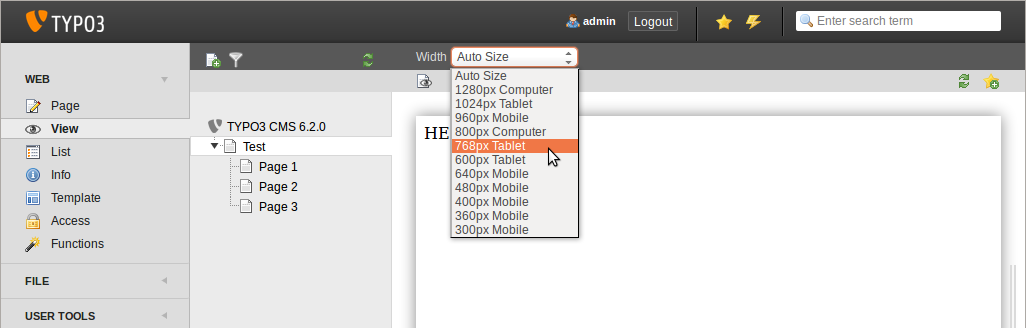
\includegraphics[width=0.95\linewidth]{Images/ResponsiveImages/ScreenSizeInPagePreview.png}
	\end{figure}

\end{frame}

% ------------------------------------------------------------------------------
% Customize Available Schermgroottes
% ------------------------------------------------------------------------------

\begin{frame}[fragile]
	\frametitle{Responsive afbeeldingen}
	\framesubtitle{Pas beschikbare schermgroottes aan}

	\begin{itemize}
		\item Schermgroottes zijn aanpasbaar via PageTSconfig:

		\lstset{
			basicstyle=\fontsize{7}{9}\selectfont\ttfamily
		}

		\begin{lstlisting}
			mod.web_view.previewFrameWidths {
			  1780.label = <any LLL or string>
			  1780.height = 145
			}
		\end{lstlisting}

		\item De breedte is gedefinieerd volgens de sleutel (hier: 1780), grootte is optioneel
		\item Voorgedefinieerde groottes kunnen worden gevonden in bestand:\newline
			\small\texttt{typo3/sysext/core/Configuration/DefaultConfiguration.php}\normalsize
		\item Labels kunnen worden gedefinieerd in PageTSconfig op de volgende manier:

		\begin{lstlisting}
			mod.web_view.previewFrameWidths {
			  1280.label = LLL:EXT:viewpage/Resources/Private/Language/locallang.xlf:computer
			  1024.label = LLL:EXT:viewpage/Resources/Private/Language/locallang.xlf:tablet
			}
		\end{lstlisting}

	\end{itemize}

\end{frame}

% ------------------------------------------------------------------------------
% Responsive Image Galleries
% ------------------------------------------------------------------------------

\begin{frame}[fragile]
	\frametitle{Responsive afbeeldingen}
	\framesubtitle{Responsive Afbeeldingen galerijen}

	\begin{itemize}
		\item Extra attributen om responsive afbeeldingen galerijen te implementeren
		\item "CSS styled content" uitgebreid om dit te bereiken
		\item Voorbeeld: HTML5 (vereist \texttt{config.doctype = html5})\newline

			TYPO3 CMS < 6.2:

			\lstset{
				basicstyle=\fontsize{7}{9}\selectfont\ttfamily
			}

			\begin{lstlisting}
				<div class="csc-textpic-imagewrap">...</div>
			\end{lstlisting}

			TYPO3 CMS >= 6.2:

			\begin{lstlisting}
				<div class="csc-textpic-imagewrap"
				  data-csc-images="{register:imageCount}"
				  data-csc-cols="{field:imagecols}">...</div>
			\end{lstlisting}

	\end{itemize}

\end{frame}

% ------------------------------------------------------------------------------
% Responsive Image Rendering
% ------------------------------------------------------------------------------

\begin{frame}[fragile]
	\frametitle{Responsive afbeeldingen}
	\framesubtitle{Responsive Image Rendering}

	\begin{itemize}
		\item cObject IMAGE rendert een "sourceCollection" om verschillende scherm dimensies te ondersteunen
		\item Responsive afbeelding rendering voor cObjects "tekst/afbeeldingen" en "afbeelding" vereist twee instellingen in de Constant Editor:

			\texttt{styles.content.imgtext.responsive}\newline
			\texttt{styles.content.imgtext.layoutKey}

		\item goede ("out of the box") opties zijn:

			\begin{itemize}
				\item \texttt{default}:	\tabto{2cm} default \texttt{<img>}-tag
				\item \texttt{srcset}:	\tabto{2cm} \texttt{<img>}-tag met alternatieve bronnen als srcset-attributen
				\item \texttt{picture}:	\tabto{2cm} \texttt{<picture>}-tag met 'ouder-kind-tags'
				\item \texttt{data}:	\tabto{2cm} \texttt{<img>}-tag met alternatieve bronnen als data-attributen 
			\end{itemize}

	\end{itemize}

\end{frame}

% ------------------------------------------------------------------------------
% Property: layoutKey
% ------------------------------------------------------------------------------

\begin{frame}[fragile]
	\frametitle{Responsive afbeeldingen}
	\framesubtitle{Property: layoutKey}

	\begin{itemize}
		\item \texttt{layoutKey} definieert rendering layout\newline
			(dit is de HTML code, gebruikt voor de\texttt{<img>}-tag)
		\item elke optie laat een ander uniek gedrag zien voor HTML rendering
		\item optie \texttt{default} rendert de \texttt{<img>}-tag traditioneel\newline
			(dit zou moeten worden gebruikt wanneer de frontend niet responsive is)
		\item Implementeren van een responsive layout vereist verschillende afbeelding dimensies voor verschillende resoluties en schermgroottes
		\item Afhankelijk van het HTML framework, de browser mogelijkheden en de JavaScript library (voor progressieve verbetering):

			\begin{itemize}
				\item gebruik een van de voorgedefinieerde layouts of
				\item definieer een eigen layout
			\end{itemize}

	\end{itemize}

\end{frame}

% ------------------------------------------------------------------------------
% Property: layout
% ------------------------------------------------------------------------------

\begin{frame}[fragile]
	\frametitle{Responsive afbeeldingen}
	\framesubtitle{Property: layout}

% *TODO* sources
% http://www.w3.org/html/wg/drafts/srcset/w3c-srcset/
% http://www.w3.org/TR/html-picture-element/

			\lstset{
				basicstyle=\tiny\ttfamily
			}

			\begin{lstlisting}
				layoutKey = {$styles.content.imgtext.layoutKey}
				layout {
				  default {
				    element = <img src="###SRC###" width="###WIDTH###" height="###HEIGHT###" ###PARAMS###
				      ###ALTPARAMS### ###BORDER######SELFCLOSINGTAGSLASH###>
				  }
				  srcset {
				    element = <img src="###SRC###" srcset="###SOURCECOLLECTION###" ###PARAMS###
				      ###ALTPARAMS### ###SELFCLOSINGTAGSLASH###>
				    source = |*|###SRC### ###SRCSETCANDIDATE###,|*|###SRC### ###SRCSETCANDIDATE###
				  }
				  picture {
				    element = <picture>###SOURCECOLLECTION###<img src="###SRC###" ###PARAMS###
				      ###ALTPARAMS######SELFCLOSINGTAGSLASH###></picture>
				    source = <source src="###SRC###" media="###MEDIAQUERY###"###SELFCLOSINGTAGSLASH###>
				  }
				  data {
				    element = <img src="###SRC###" ###SOURCECOLLECTION### ###PARAMS###
				      ###ALTPARAMS######SELFCLOSINGTAGSLASH###>
				    source = data-###DATAKEY###="###SRC###"
				  }
				}
			\end{lstlisting}

\end{frame}

% ------------------------------------------------------------------------------
% Property: layout.[layoutKey].element
% ------------------------------------------------------------------------------

\begin{frame}[fragile]
	\frametitle{Responsive afbeeldingen}
	\framesubtitle{Property: layout.[layoutKey].element}


	\begin{itemize}
			\item \lstinline!###SRC###!\newline
				URL voor het attribuut: \texttt{src}

			\item \lstinline!###WIDTH###!\newline
				Afbeelding breedte (in pixel) voor het attribuut: \texttt{width}

			\item \lstinline!###HEIGHT###!\newline
				Afbeelding hoogte (in pixel) voor het attribuut: \texttt{height}

			\item \lstinline!###PARAMS###!\newline
				Extra parameters zoals gedefinieerd in cObject IMAGE

			\item \lstinline!###ALTPARAMS###!\newline
				Extra alternatieve parameters zoals gedefinieerd in cObject IMAGE

	\end{itemize}

\end{frame}

% ------------------------------------------------------------------------------
% Property: layout.[layoutKey].element
% ------------------------------------------------------------------------------

\begin{frame}[fragile]
	\frametitle{Responsive afbeeldingen}
	\framesubtitle{Property: layout.[layoutKey].element}

		\begin{itemize}
			\item \lstinline!###BORDER###!\newline
				Rand (in pixel) voor het attribuut: \texttt{border}

			\item \lstinline!###SELFCLOSINGTAGSLASH###!\newline
				Afsluitende tag, e.g. \texttt{<img ... />} vs. \texttt{<img ... >}\newline
				(afhankelijk van \texttt{config.xhtmlDoctype} of \texttt{config.doctype})

			\item \lstinline!###SOURCECOLLECTION###!\newline
				Extra afbeelding bronnen, afhankelijk van het gebruik van responsive web design.
				Exacte waardes zijn gedefinieerd in de sleutel: \texttt{layout.[layoutKey].source}

	\end{itemize}

\end{frame}

% ------------------------------------------------------------------------------
% Property: sourceCollection.[dataKey]
% ------------------------------------------------------------------------------

\begin{frame}[fragile]
	\frametitle{Responsive afbeeldingen}
	\framesubtitle{Property: sourceCollection.[dataKey]}

	\begin{itemize}
		\item Standaard sourceCollection van EXT:css\_styled\_content
		\item het schrijven van je eigen sourceCollection is eigenlijk een vereiste en daarom zeer aan te raden
		\lstset{
				basicstyle=\tiny\ttfamily
			}

			\begin{lstlisting}
				sourceCollection {
				  small {
				    width = 200
				    srcsetCandidate = 600w
				    mediaQuery = (max-device-width: 600px)
				    dataKey = small
				  }
				  smallRetina {
				    if.directReturn = 1
				    width = 200
				    pixelDensity = 2
				    srcsetCandidate = 600w 2x
				    mediaQuery = (max-device-width: 600px) AND (min-resolution: 192dpi)
				    dataKey = smallRetina
				  }
				}
			\end{lstlisting}
	\end{itemize}

\end{frame}

% ------------------------------------------------------------------------------
% Further Resources (External Links)
% ------------------------------------------------------------------------------

\begin{frame}[fragile]
	\frametitle{Responsive afbeeldingen}
	\framesubtitle{Verdere bronnen}

	\begin{itemize}
		\item Werkend voorbeeld van de code hier:\newline
			\small\url{http://wiki.typo3.org/Responsive_Image_Rendering}\normalsize

		\item Artikel van Sven Wolfermann op typo3.org:\newline
			\small\url{http://typo3.org/news/article/responsive-image-rendering-in-typo3-cms-62/}\normalsize

		\item Werkende test van de "Responsive Image Community Group":\newline
			\small\url{http://responsiveimages.org}\normalsize

	\end{itemize}

\end{frame}

% ------------------------------------------------------------------------------

